\chapter{Conclusion}
\epigraph{Of what a strange nature is knowledge! It clings to a mind when it has once seized on it like a lichen on a rock.}{\textsc{Mary Shelley}, \textit{Frankenstein; or, The Modern Prometheus}}


And thus, we have reached the end. This dissertation has dealt with the development of a general framework for improving the performance of model-based visual odometry pipelines through learned probabilistic pseudo-sensors that extract difficult-to-model latent information.  We presented four examples of such \textit{pseudo-sensors}. We close with a final summary of the contributions and list of publications, a discussion of potential future work, and some concluding remarks.

\section{Summary of Contributions}

\subsection{Predictive Robust Estimation}

\begin{wrapfigure}{r}{0.3\textwidth}
  \begin{center}
  	\vspace{-25pt}
    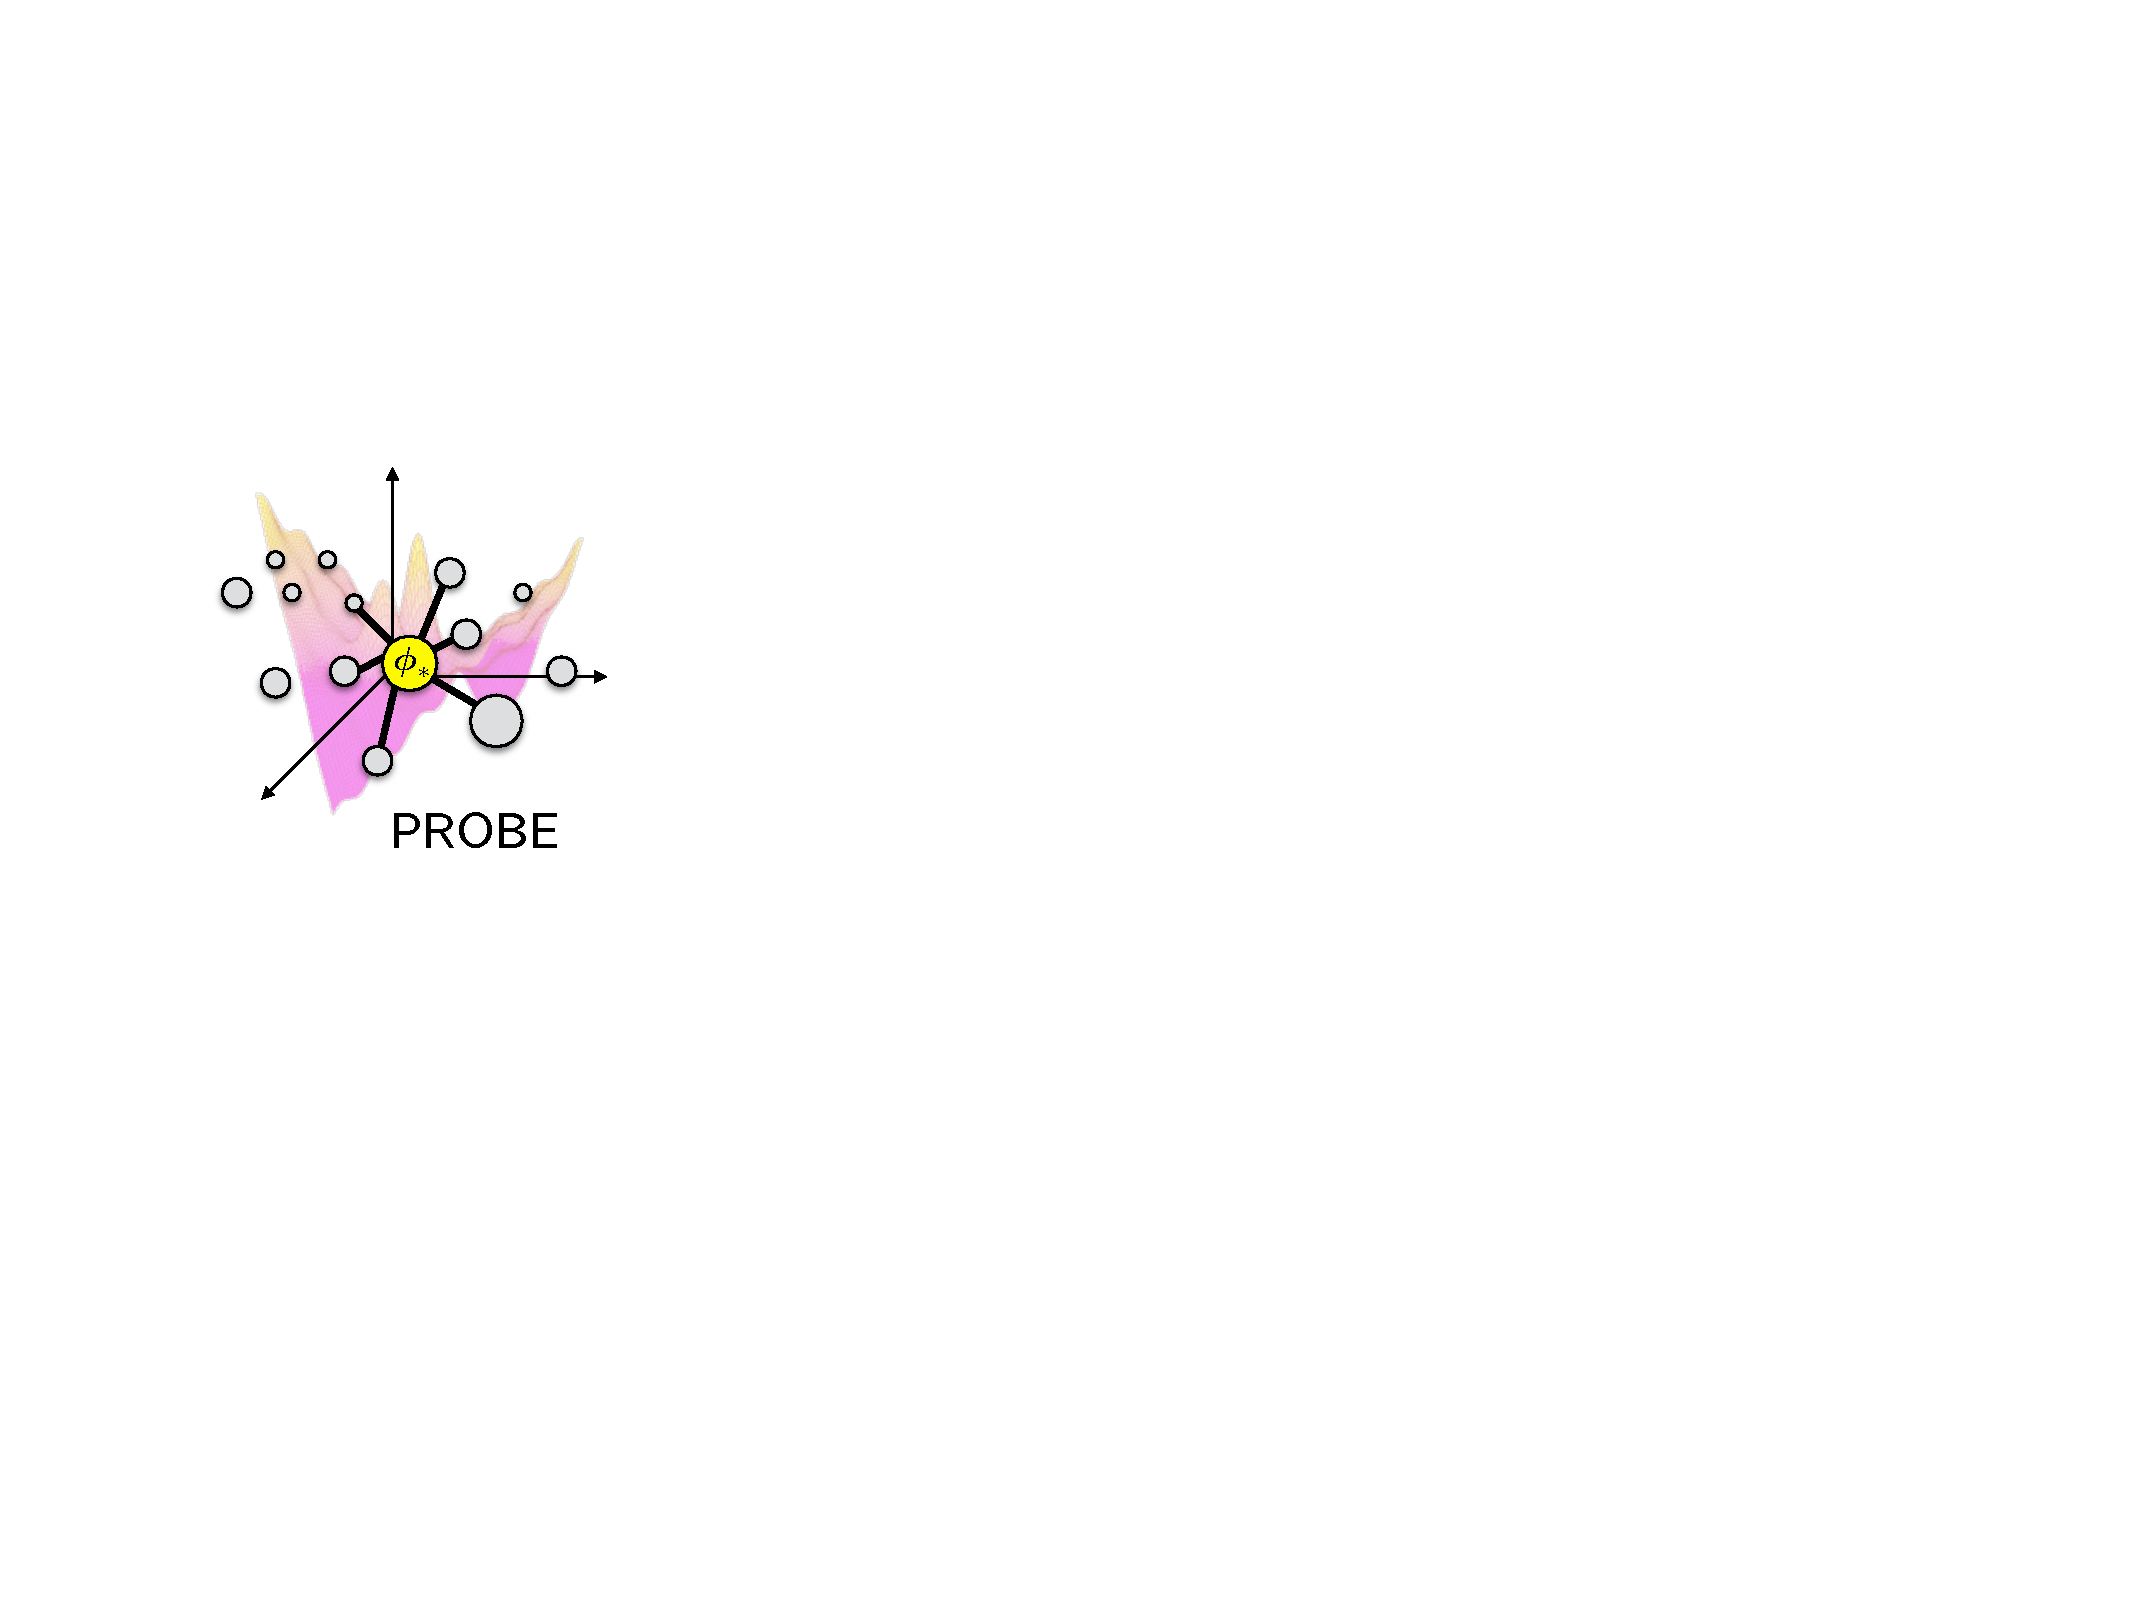
\includegraphics[width=0.28\textwidth]{conclusion/probe}
     \vspace{-25pt}
  \end{center}
  \caption{PROBE (\Cref{ch:probe}).}
  \vspace{-5pt}
\end{wrapfigure}


We began with a pseudo-sensor that used a heteroscedastic noise model to enable predictively robust estimation. PROBE and its follow-up work, PROBE-GK, contributed
\begin{enumerate}
\item a probabilistic model for indirect stereo visual odometry, leading to a predictive robust algorithm for inference on that model,
\item two different approaches to constructing the robust algorithm: one baseds on k-nearest neighbours, and one based on Generalized Kernel (GK) estimation,
\item a procedure for training our model using pairs of stereo images with known relative transforms, and
\item an iterative, expectation-maximization approach to train our GK model when the relative ground truth egomotion was unavailable.
\end{enumerate}

%\noindent A total of three publications associated with PROBE,
%\begin{itemize}
%	\item \bibentry{2016_Peretroukhin_PROBE-GK}
%	\item \bibentry{2015_Peretroukhin_PROBE}
%	\item \bibentry{2015_Peretroukhin_Get}.
%\end{itemize}


\subsection{Sun BCNN}

\begin{wrapfigure}{r}{0.3\textwidth}
  \begin{center}
  	\vspace{-20pt}
    
\includegraphics[width=0.28\textwidth]{conclusion/sun_bcnn}
     \vspace{-15pt}
  \end{center}
  \caption{Sun BCNN (\Cref{ch:sun-bcnn}).}
  \vspace{-5pt}
\end{wrapfigure}


With Sun-BCNN, we applied learned \textit{pseudo-sensors} to the problem of illumination direction in outdoor environments. In sum, the novel contributions were:
\begin{enumerate}
\item the application of a Bayesian CNN to the problem of sun direction estimation, incorporating the resulting covariance estimates into a visual odometry pipeline; 
\item an empirical demonstration that a Bayesian CNN with dropout layers after each convolutional and fully-connected layer can achieve state-of-the-art accuracy at test time;
\item a loss function that incorporated a 3D unit-length sun direction vector, appropriate for full 6-DOF pose estimation;
\item experimental results on over 30~km of visual navigation data in urban \citep{Geiger2012-fq} and planetary analogue \citep{Furgale2012-kk} environments; 
\item an investigation into the sensitivity of the Bayesian CNN-based sun estimate to cloud cover, camera and environment changes, and measurement parameterization; and
\item open-source software\footnote{\url{https://github.com/utiasSTARS/sun-bcnn-vo}.}.
\end{enumerate}

%\noindent Sun-BCNN and its origin in learned sun sensors have three associated publications,
%\begin{itemize}
%	\item \bibentry{2018_Peretroukhin_Inferring}
%	\item \bibentry{2017_Peretroukhin_Reducing}
%	\item \bibentry{2017_Clement_Improving}.
%\end{itemize}


\subsection{Deep Pose Corrections}

\begin{wrapfigure}{r}{0.3\textwidth}
  \begin{center}
  	\vspace{-20pt}
    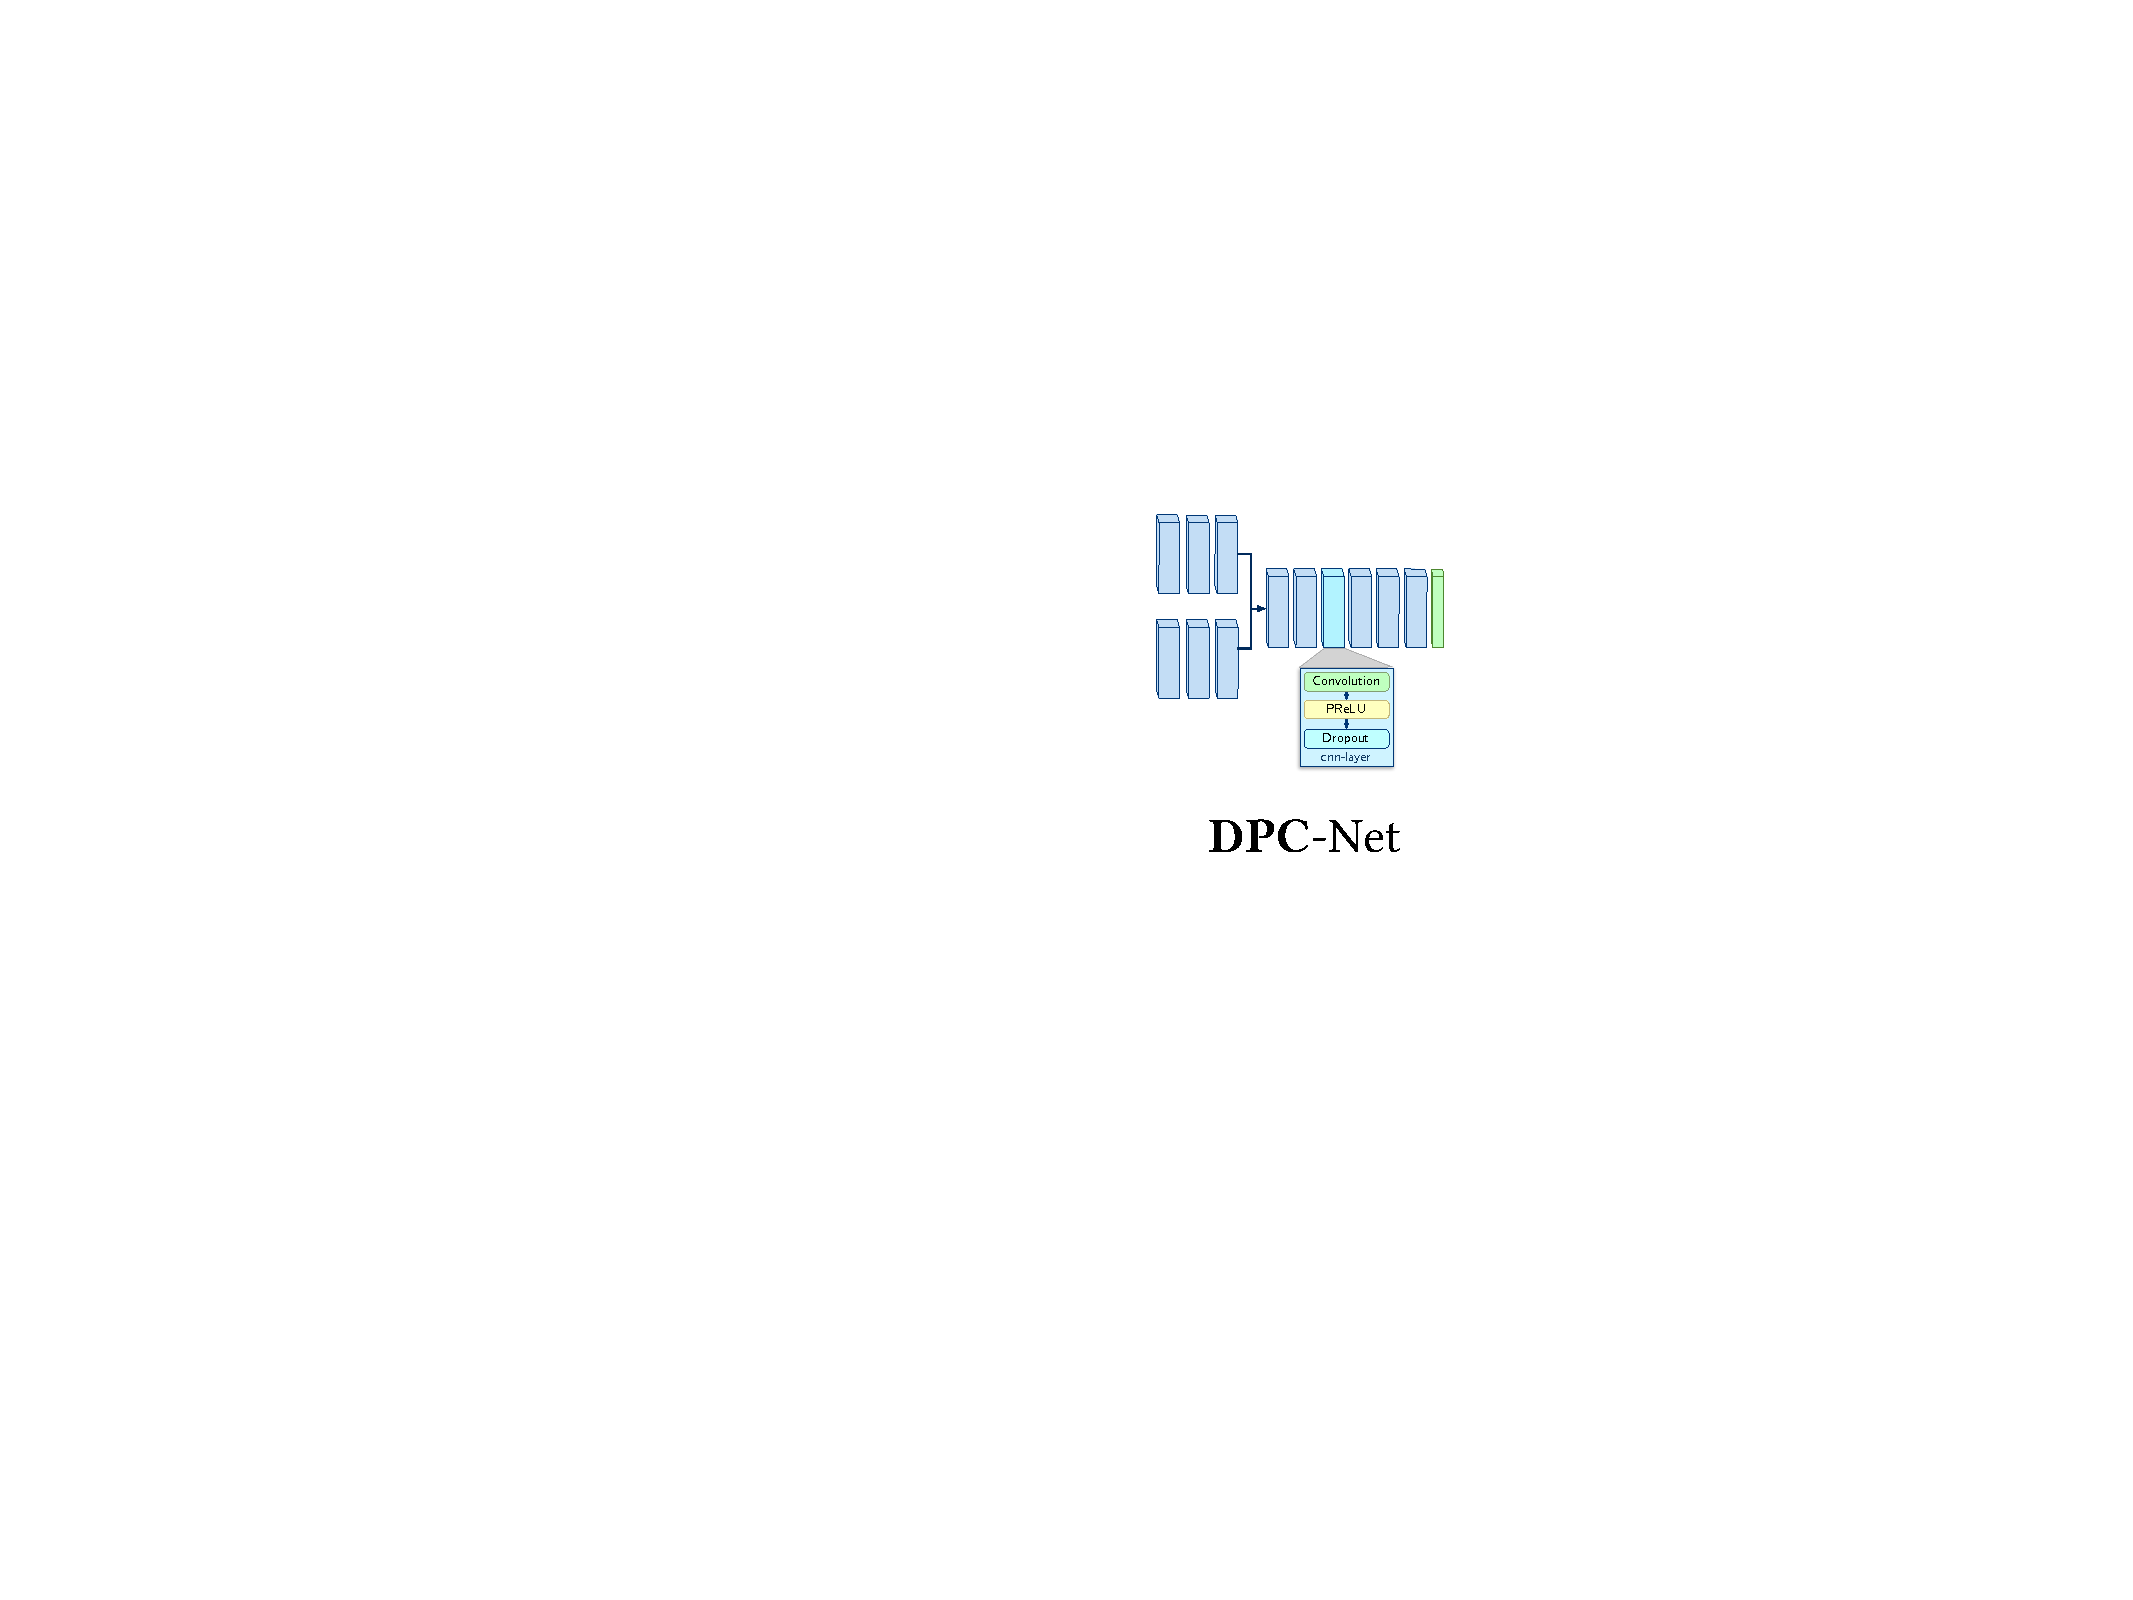
\includegraphics[width=0.28\textwidth]{conclusion/dpc}
     \vspace{-15pt}
  \end{center}
  \caption{DPC-Net (\Cref{ch:dpc}).}
  \vspace{-5pt}
\end{wrapfigure}


Next, we generalized the results of Sun-BCNN to learn full six degree-of-freedom corrections for a particular egomotion pipeline and a given environment with DPC-Net. Our contributions included

\begin{enumerate}
	\item the formulation of a novel deep corrective approach to egomotion estimation,
	\item a novel cost function for deep $\LieGroupSE{3}$ regression that naturally balances translation and rotation errors, and
	\item an open-source implementation of DPC-Net in \texttt{PyTorch}\footnote{See \url{https://github.com/utiasSTARS/dpc-net}.}.
\end{enumerate}

%\noindent DPC-Net was published in a journal publication,
%\begin{itemize}
%	\item \bibentry{2018_Peretroukhin_Deep}.
%\end{itemize}


\subsection{Deep Probabilistic Inference of $\LieGroupSO{3}$ with HydraNet}

\begin{wrapfigure}{r}{0.3\textwidth}
  \begin{center}
  	\vspace{-20pt}
    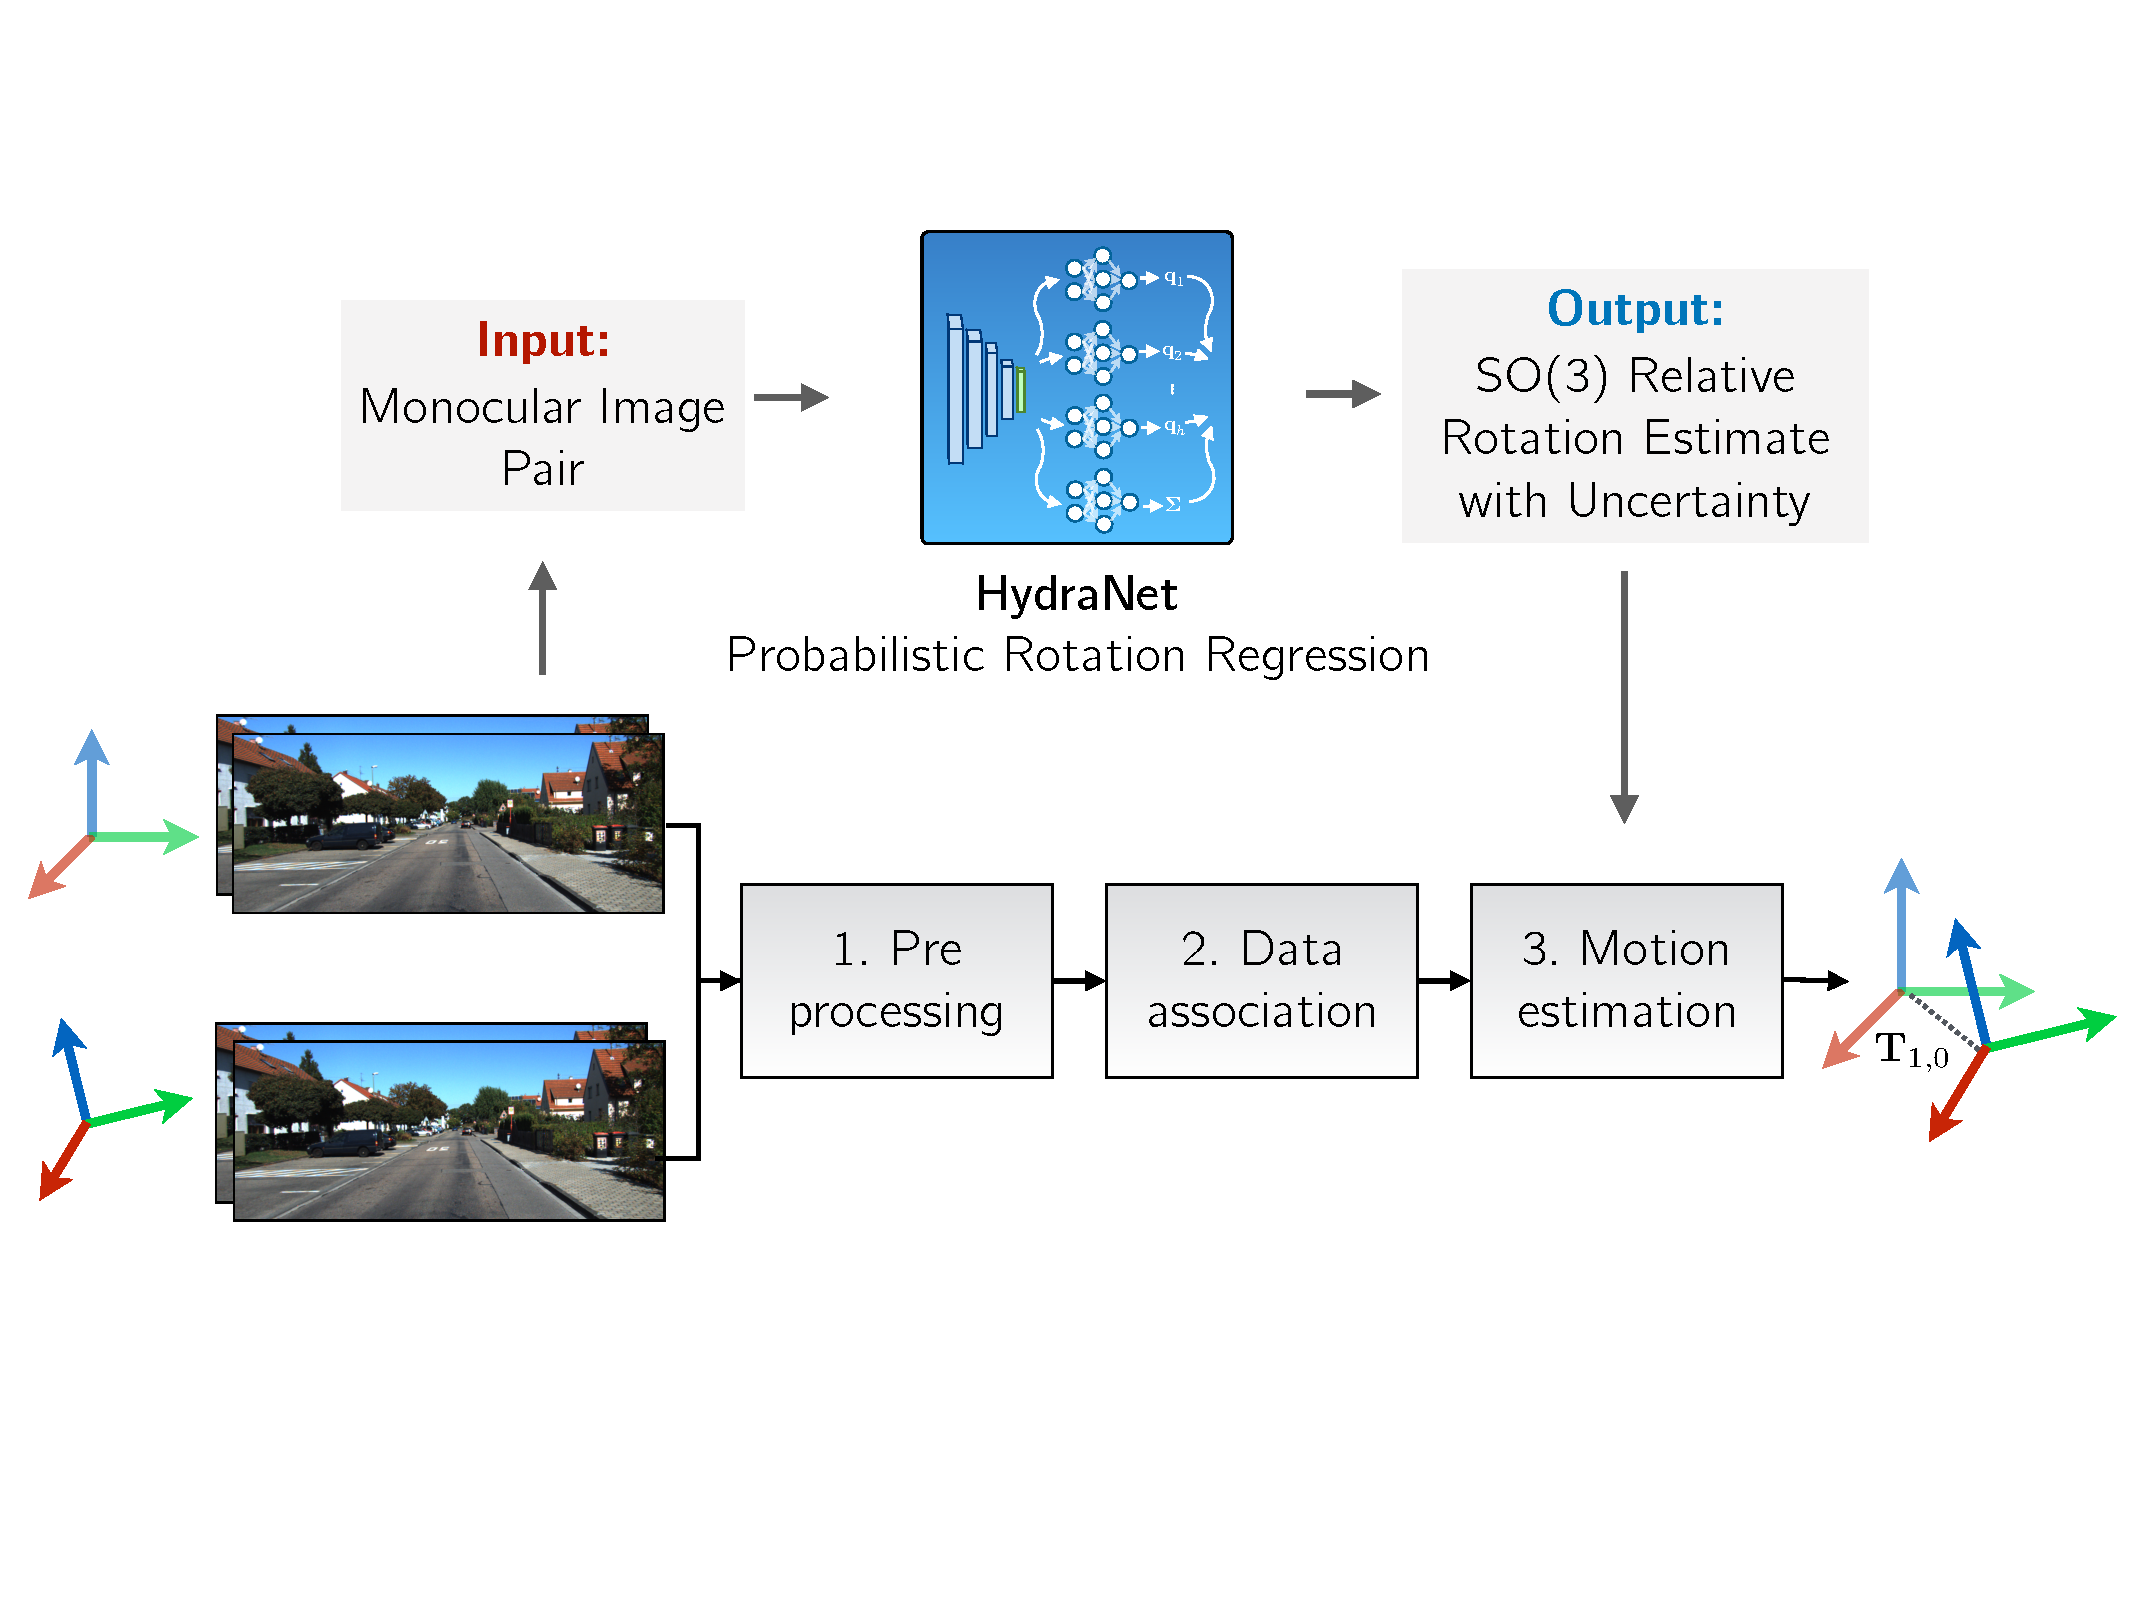
\includegraphics[width=0.28\textwidth]{conclusion/hydranet}
     \vspace{-15pt}
  \end{center}
  \caption{HydraNet (\Cref{ch:hydranet}).}
  \vspace{-5pt}
\end{wrapfigure}


Finally, we applied the lessons of DPC-Net and Sun-BCNN to learning only rotation estimates through a network structure that incorporated both aleatoric and epistemic uncertainty which can be fused with classical pipelines through pose graph optimization. With this work, we contributed
\begin{enumerate}
\item a deep network structure we call \textit{HydraNet} that built on prior work \cite{Lakshminarayanan2017,Osband2016} to produce meaningful uncertainties over unconstrained targets,
\item a loss formulation and mathematical framework that extends HydraNet to means and covariances of the rotation group $\LieGroupSO{3}$,
\item and open source code for $\LieGroupSO{3}$ regression\footnote{\url{https://github.com/utiasSTARS/so3_learning}.}.
\end{enumerate}

%\noindent HydraNet was published in a refereed workshop paper,
%\begin{itemize}
%\item \bibentry{2019_Peretroukhin_Deep}.
%\end{itemize}


\section{Future Work}

\begin{figure}
\begin{center}
		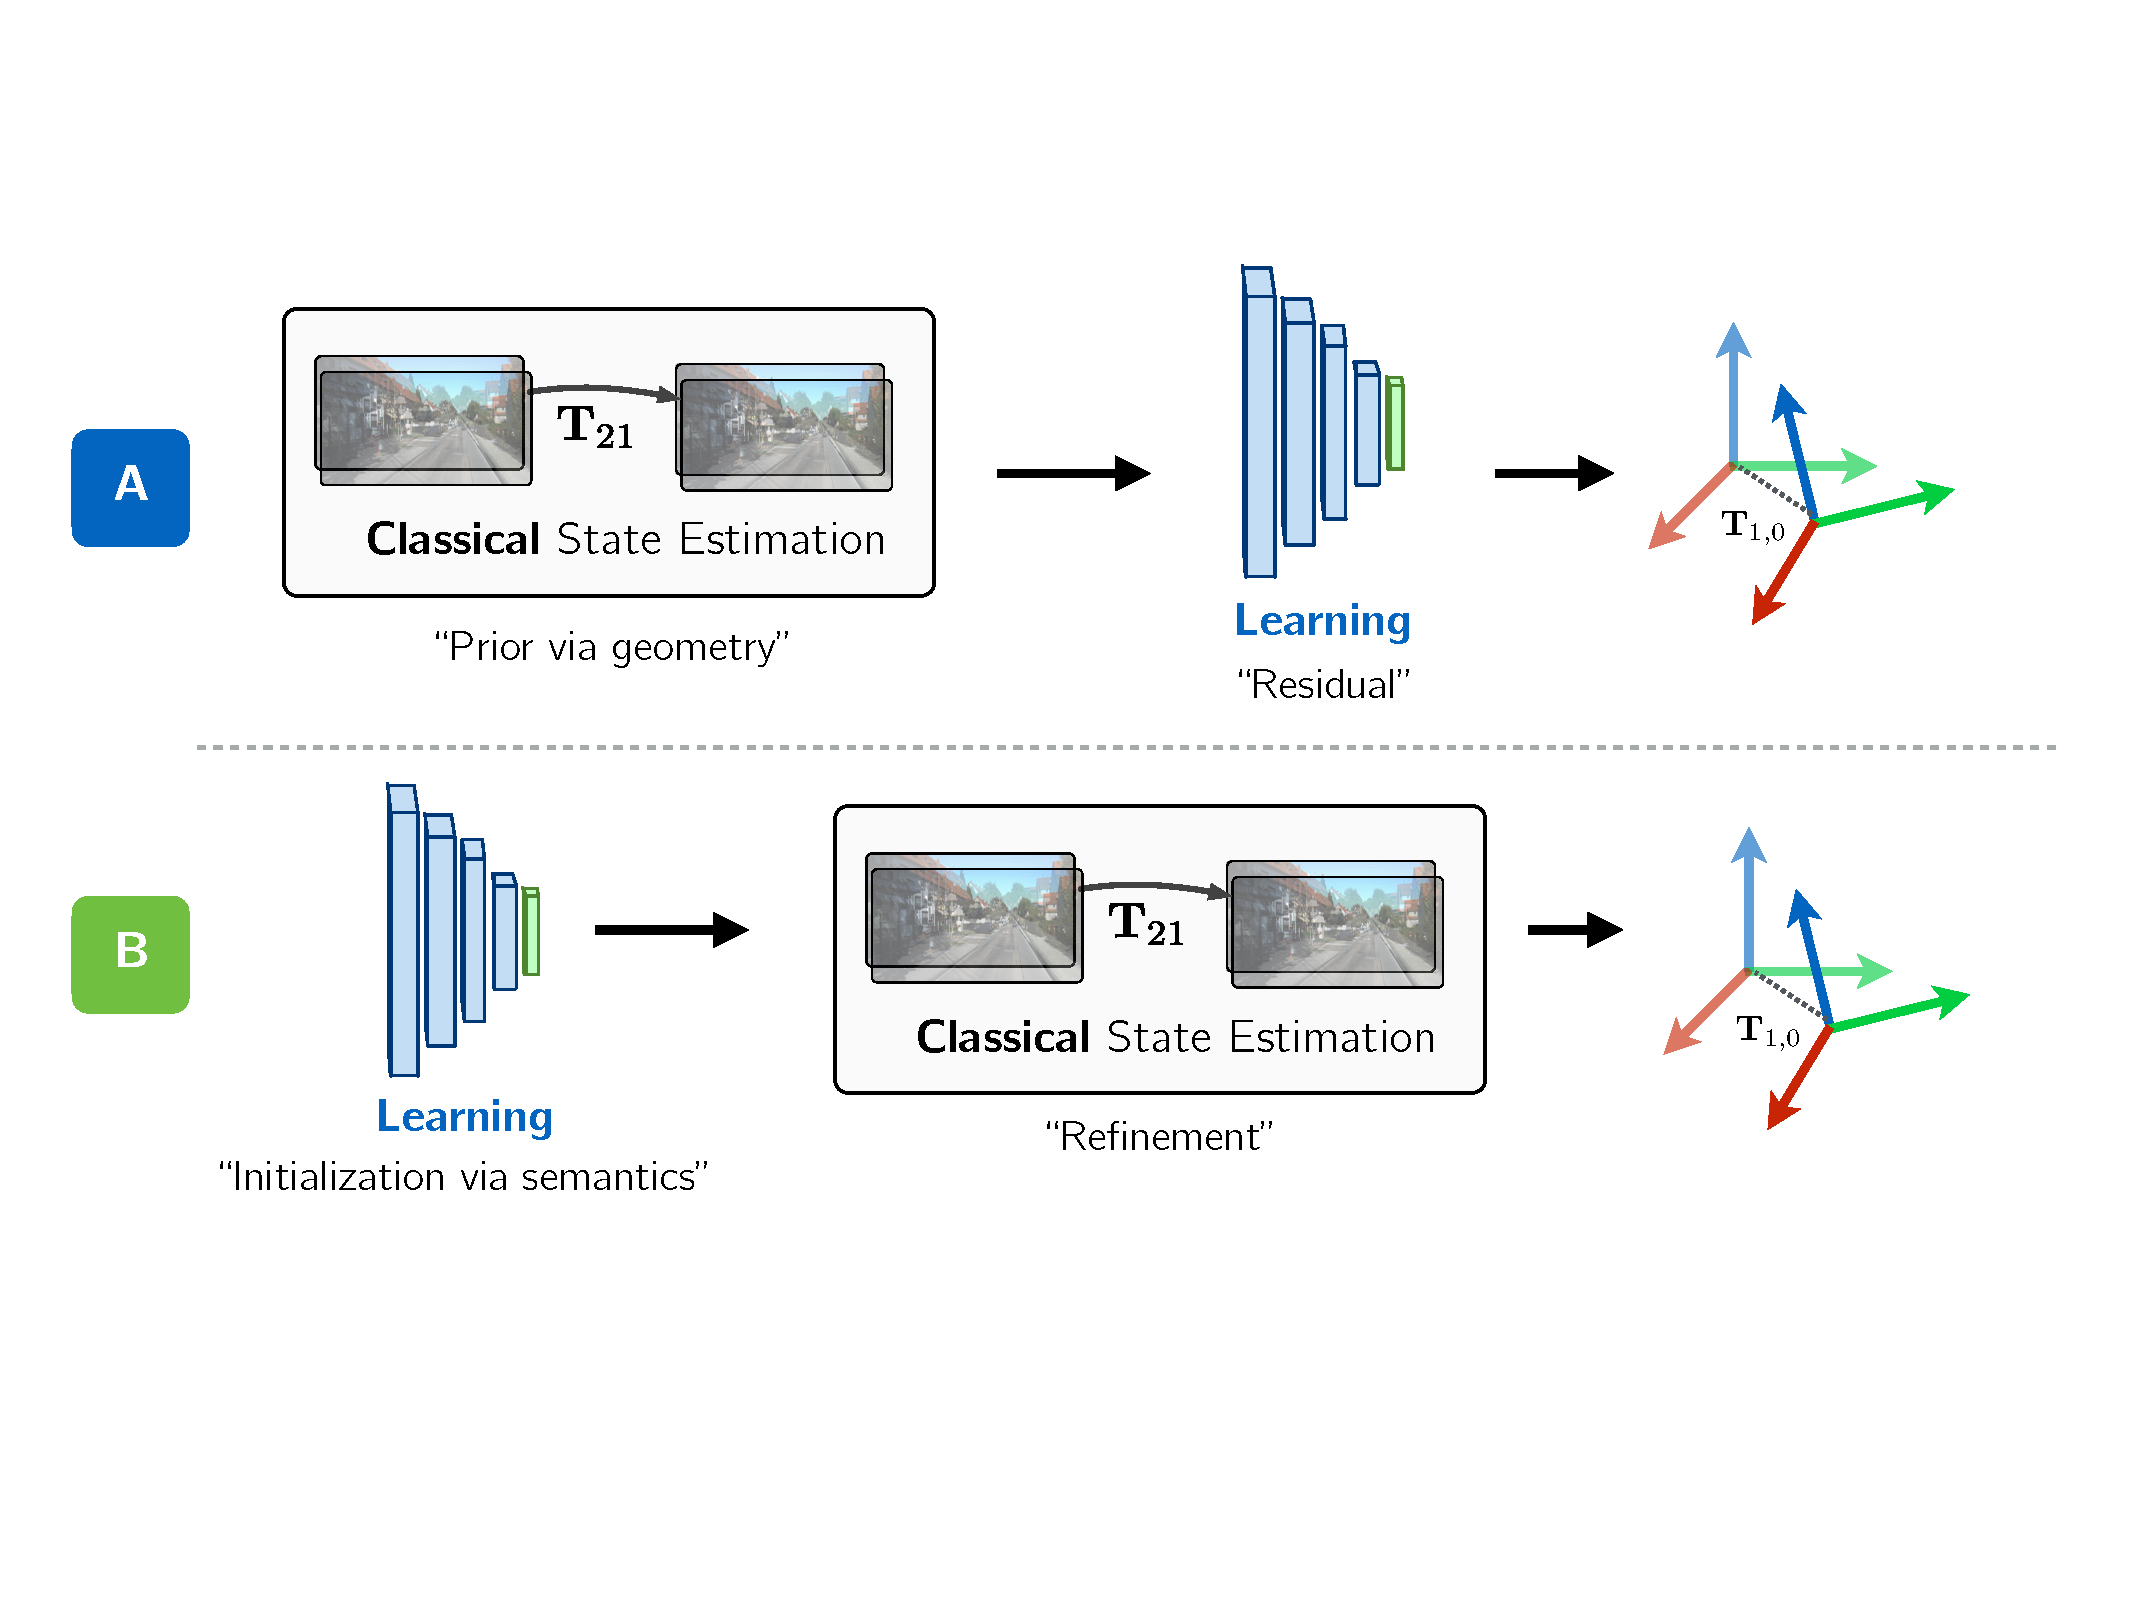
\includegraphics[width=0.98\textwidth]{conclusion/learning_as_prior.pdf}
		\caption{Two different ways to incorporate learning with classical pipelines. The first is by using pipelines as a \textit{prior} which can then be corrected by learned approaches, while the second is use learning as an initialization which can then be \textit{refined} by classical techniques.}
  	\label{fig:conc_learning_as_prior}
\end{center}
\end{figure}


There are many avenues for future work. For instance, although the fusion of pipelines with pseudo-sensors can significantly improve localization performance in a given environment, there are few guarantees that the final estimates are accurate and consistent.

A potential thread of future work addresses this deficiency by developing more tightly-coupled perception systems that can be ‘certified’ to produce globally-optimal solutions while still being robust to adverse environmental effects. To do this, we propose that another way to fuse learned models with classical optimization techniques. Instead of treating the learning as a way to incorporate residuals (as much of this thesis is), we propose that we use learning as initializations, or priors, that are more invariant to effects like large view-point changes and have the ability to generalize to large-scale environments (\Cref{fig:conc_learning_as_prior}). By incorporating these learned ‘priors’ into an optimization framework, we can leverage recently-developed theory on convex relaxations (e.g., that presented in \cite{Rosen2019-kk}) to ensure that the final localization and mapping results are ‘optimal’, in the sense that they are the global minima of a maximum-likelihood-based loss, and ‘safe’, in the sense that they provide consistent uncertainty estimates even in the presence of unmodelled effects. 

\section{Final Remarks}

The German Philosopher Georg Hegel had a particular dialectic method that involved a triad: a thesis, antithesis and synthesis.
Somewhat curiously, this \textit{thesis} has been an attempt at a \textit{synthesis} of the thesis posed by classical visual egomotion, and the antithesis posed by data-driven end-to-end learning techniques.
My hope is that the synthesis proposed by the paradigm of learned \textit{pseudo-sensors} will prove to be a fruitful one within the field of state-estimation, and for the broader robotics community at large. 

\section{Coda: In Search of Elegance}
\epigraph{Machinery that gives us abundance has left us in want.
Our knowledge has made us cynical.
Our cleverness, hard and unkind.
We think too much, and feel too little.
More than machinery, we need humanity.}{\textsc{Charlie Chaplin}, \textit{The Great Dictator}}

%A fascination on machines to a fascination with people
%Data-driven learning is in many ways humans waving the white flag to the overwhelming complexity of the world
%We relinquish the dream of simplification and interpretation 
%And instead we are satisfied with only prediction
%Hubris of 'hand design'
%Puppeteers and roboticists
%In search of elegance

Looking back on my academic journey, I see a path from a fascination with the possible applications of autonomous systems to a fascination with autonomy \textit{in-and-of-itself}. As a budding researcher, I saw robust, accurate perception as a means towards an end. An end which entailed truly autonomous systems `perceiving' and `interpreting' their surroundings with the goal of exploring distant planets and navigating busy urban streets. Now, however, I see `perception' as an end in itself with a plethora of fascinating mathematical, philosophical and ethical challenges that can be tackled in light of, but not subservient to, the potential goals of some grander autonomous system. Throughout this transition, I have become more interested not only in the flesh and blood of perception systems, but also in the \textit{spirit} of them. If perception is one of the bridges we must build to reach the land of autonomy, I am concerned not only with the structural integrity that lets us cross it today, but also with an elegance and rigour that lets it serve as model for posterity. 

With this in mind, I want to address a concerning shift that has occurred in the research community throughout my academic career. Many researchers who work on algorithms that enable autonomy (not only in perception, but also in planning and controls) have given up on the dream of modelling the world with the tools of Euclid, Newton and Euler in favour of methods that rely on exemplary data to `train' arbitrarily complex predictive black-box models. In my estimation, this shift has brought with it a certain sense of resignation to the overwhelming complexity of the world. Researchers (including yours truly) are often content to use vague notions of complexity as reason to avoid building analytic models. Instead, we turn to high-parameter data-efficient crude surrogates of our own brains to model what we do not want to. This, I believe, is a tempting mistake. Although these solutions may serve as useful tools to temporarily bridge gaps in our understanding of the world, we will inevitably deplete the low-hanging empirical fruits that they can bear, and we will be left with a deep sense of dissatisfaction that only elegance and simplicity can fill. 

I am certainly not the first or the last person who has taken issue with data-driven methods. Noam Chomsky gives the following critique of purely statistical approaches to science\footnote{\url{http://norvig.com/chomsky.html}}. Consider the study of bee colonies. In order to to extract interpretable models of their behaviour (e.g., there is a queen bee, there are worker bees, etc.), one has to observe these colonies meticulously over generations. So why not avoid that entire endeavour and use a data-driven approach? We could set up a camera to observe a bee colony and collect data over several years. By tracking each bee, we could use the tools of modern machine learning to construct and train a large parametric model of each of their positions. Once complete, we could then query this model with a new image from our camera and recover, with extreme precision, the predicted location of each bee. This may allow us to improve honey production, but what have we learned? Is this an elegant model of bee behaviour? Have we not just transformed the problem of understanding the bees into one of understanding this surrogate model? Now consider doing the same with celestial objects--Kepler be damned!

Some may argue that the entire goal of science is predicting the future states of nature, so elegance is irrelevant. I vehemently disagree. I would rather have an interpretable model that is wrong during specific situations (where I can verify that certain assumptions are violated), rather than an obfuscated model which has vague limits to its predictive power.

If history is any judge, the models that stand the test of time are ones that are born out of our meticulous labour and enlightened insight to extract salient principles out of the complexity of the world. The hope that this labour can be replaced with black-box surrogates that indirectly learn these same principles is troubling and, in my view, unnecessary. No matter how much anthropomorphic language we use to describe these surrogates (endowing them with `understanding', `attention', and `forgetfulness'), they will always be limited by our own ability to collect sufficient data, and by our ability to craft them in such a way as to consume significant amounts of training exemplars without `overfitting' to them. What's more, if these models have any interaction with the world, they will also affect the world, and we are committing ourselves to an endless game of cat-and-mouse. Although it may seem that our time is best spent crafting ever-more-clever surrogates, we will soon reach a point where we would be better off using the time and resources towards studying a particular problem more directly.

I do not want to cast aspersions flippantly.  The transition to data-driven approaches in computer vision happened for good reason and with much hesitation. The elegance of analytic models has historically only been exceeded by their inability to model the often inelegant `real world'. As late as 2006, roboticists were joking that the dirty secret of computer vision is that it doesn't work. Recent efforts into combining the connectionist ideas of the 20th century with the computational power accessible in the 21st have undoubtedly created systems that do attain impressive empirical results, and there is a constant stream of new theoretical insights into the types of networks and optimization methods that work well in a given domain.

However, as the world becomes more connected and complex with every passing day, I think it is of utmost importance that autonomy researchers are not tempted to focus solely on empirical results at the cost of elegant solutions. It is now well-accepted that data-driven methods are not the panacea (like it might have seemed for a brief moment a few years ago) to all problems in autonomy. However, this passive agreement may not be enough. Instead, we need to actively suppress the urge to try and solve a problem first through general `learning' methods that are becoming more and more easy to implement and less and less easy to understand.  We do not need to relinquish the dream of understanding the world and relegate ourselves to simply predicting it by any means possible. We can instead strive to simplify it and interpret it. If after significant effort we fail at that goal, and only then, should we turn to data-driven learned models to fill in the gaps in our understanding.

